% Основная часть
\section{Аналитическая часть}

\noindent
\hspace{0.75cm}
В данном разделе проведена формализация задачи, формализация данных, анализ баз данных и систем управления базами данных, подходящих для данной задачи.

\subsection{Формализация задачи}

\noindent
\hspace{0.75cm}
Дана трубка, представленная набором сечений, каждое из которых состоит из точек $P_i = {p_{i1}, p_{i2}, ..., p_{in_i}}$, соединенных с несколькими другими точками, в том числе из соседних сечений. Каждая точка $p_{ij}$ имеет координаты $(x_{ij}, y_{ij}, z_{ij})$.

\noindent
\hspace{0.75cm}
Пользователь выбирает точку, относительно которой будет происходить деформация и направление деформации. Во время деформации трубки, история сечений будет сохраняться в базу данных. Деформация будет происходить по следующему закону: (здесь будет формализация модели деформации).

\subsection{Формализация данных}

\noindent
\hspace{0.75cm}
Основываясь на сформулированных требованиях, база данных должна содержать информацию об:

\begin{itemize}
	\item историю деформации трубки;
	\item деформируемой трубке;
	\item сечениях, содержащихся в трубке;
	\item точках, составляющих сечение;
	\item ребрах, соединяющих пары точек;
	\item пользователях.
\end{itemize}

\noindent
\hspace{0.75cm}
Связи между описанными сущностями представлены на ER-диаграмме (рисунок~\ref{fig:er}).

\begin{figure}[H]
\centering
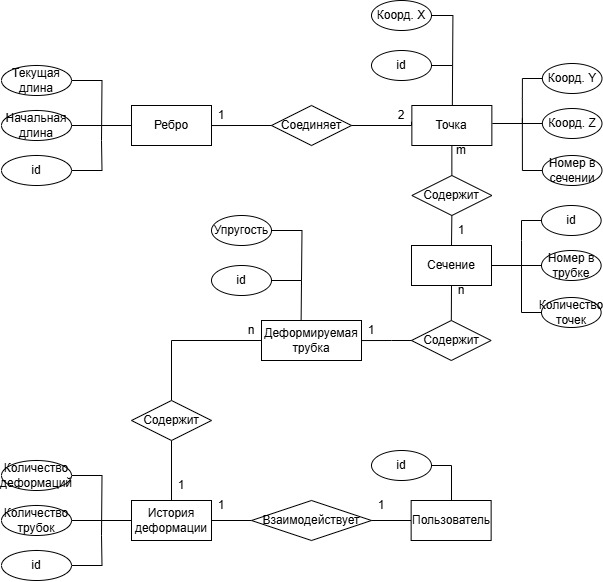
\includegraphics[width=1.05\textwidth]{img/er_диаграмма.jpg}
\caption{ER-диаграмма сущностей}
\label{fig:er}
\end{figure}

\subsection{Пользователь}

\noindent
\hspace{0.75cm}
В рамках данной курсовой работы выделена одна роль пользователя приложением. Пользовательские Use-case представлены на рисунке~\ref{fig:use-case}.

\begin{figure}[H]
\centering
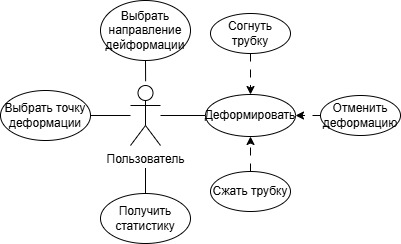
\includegraphics[width=0.9\textwidth]{img/use-case.jpg}
\caption{Use-case-диаграмма}
\label{fig:use-case}
\end{figure}

\subsection{Выбор модели данных}

\noindent
\hspace{0.75cm}
Модель данных~---~это совокупность абстракций и методов, с помощью которых мы стремимся имитировать понятия реального мира~\cite{komarov}.

\subsubsection{Реляционная модель}

\noindent
\hspace{0.75cm}
Реляционные СУБД (такие как PostgreSQL, MySQL, Oracle) основаны на реляционной модели данных, где информация организуется в таблицы, состоящие из строк и столбцов. Каждая таблица имеет определенную структуру, а связи между таблицами устанавливаются с помощью внешних ключей~\cite{vas_hus}.

\subsubsection{Документо-ориентированная модель}

\noindent
\hspace{0.75cm}
Документо-ориентированные СУБД (MongoDB, CouchDB) хранят данные в виде документов, обычно в формате JSON. Каждый документ содержит пары ключ-значение и может иметь вложенную структуру~\cite{luchinina}.

\subsubsection{База данных временных рядов}

\noindent
\hspace{0.75cm}
БД временных рядов специализированы для хранения последовательных событий или измерений с временными метками~\cite{komarov}.

\subsubsection{Объектно-ориентированная модель}

\noindent
\hspace{0.75cm}
Объектная модель БД строится на принципах объектно-ориентированного программирования, где данные хранятся в виде объектов с методами~\cite{eldar}.

\subsubsection{Графовые базы данных}

\noindent
\hspace{0.75cm}
Графовые СУБД (Neo4j, OrientDB, ArangoDB) специализируются на хранении связей между объектами. Данные представляются в виде узлов (вершин) и связей между ними (рёбер), что обеспечивает естественное представление сетевых структур~\cite{otradnov}.
